  %%%%%%%%%%%%%%%%%%%%%%%%%%%%%%%%%%%%%%% -*- coding: utf-8; mode: latex -*- %%
  %
%%%%%                         CHAPTER
 %%%
  %

% $Id: 1020-lorem-ipsum.tex,v 1.2 2009/06/19 15:51:46 david Exp $
% $Log: 1020-lorem-ipsum.tex,v $
% Revision 1.2  2009/06/19 15:51:46  david
% *** empty log message ***
%
% Revision 1.1  2007/11/23 09:52:39  david
% *** empty log message ***
%
%

  %%%%%%%%%%%%%%%%%%%%%%%%%%%%%%%%%%%%%%%%%%%%%%%%%%%%%%%%%%%%%%%%%%%%%%%%%%%%%
  %
%%%%%                           HEAD MATTER
 %%%
  %

\chapter{Read-Only Nested Snapshots Implementation and Evaluation}
%\addcontentsline{lof}{chapter}{\thechapter\quad Lorem Ipsum}
%\addcontentsline{lot}{chapter}{\thechapter\quad Lorem Ipsum}
\label{ch:RORLSSIE}
The algorithm to list subtree of directory at a given snapshot was implemented in SQl and executed against MySql NDB cluster. 
\section{Benchmark for measuring query execution time}
In this benchmark, a single directory with 1,000,000 files is used as test directory. Snapshot is taken when vector clock is 5000 i.e after completion 5000 operation. Following operations are executed on the test directory.
\begin{enumerate}
\item \textbf{ADD :} Adding new files to the directory
\item \textbf{DEL:} Deleting exisiting files in the directory
\item \textbf{RENAME:} Renaming exisiting files in the directory
\item \textbf{MOV:} Moving file from this directory to another directory.
\item \textbf{MOV\_ IN:} Moving back the files that were moved out in MOV operation.
\item \textbf{Time:} Time taken for executing listing files in the directory at snapshot taken at time 5000.
These measurements are taken on ndb cluster while the query executed at MySql server instead of clusterj.
\end{enumerate}
\begin{figure}[tbh]
\centering  
 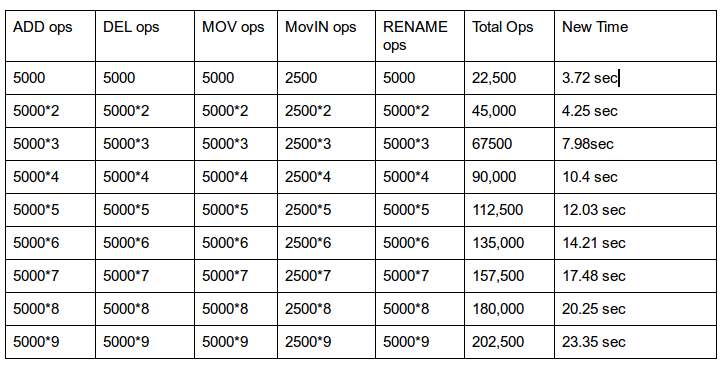
\includegraphics[scale=0.8]{figs/preliminar/Benchmark1.png}
  \caption{Benchmark on Single Directory}
  \label{fig:Benchmark1}
\end{figure}
\begin{figure}[tbh]
\centering  
 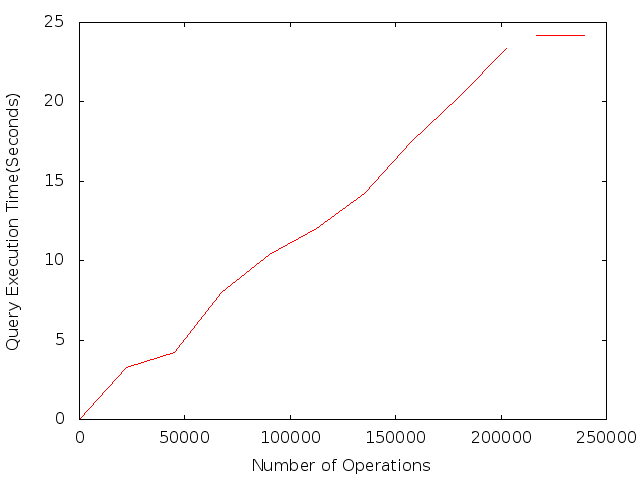
\includegraphics[scale=0.5]{figs/preliminar/benchmark_graph2.png}
  \caption{Benchmark on Single Directory Graph}
  \label{fig:benchmark_graph2}
\end{figure}

The benchmark shows that the execution time scales linearly with the number of operations.


  %%%%%%%%%%%%%%%%%%%%%%%%%%%%%%%%%%%%%%%%%%%%%%%%%%%%%%%%%%%%%%%%%%%%%%%%%%%%%
  %
%%%%%                        FIRST SECTION
 %%%
  %




  %%%%%%%%%%%%%%%%%%%%%%%%%%%%%%%%%%%%%%%%%%%%%%%%%%%%%%%%%%%%%%%%%%%%%%%%%%%%%
  %
%%%%%                         ANOTHER SECTION
 %%%
  %


  %
 %%%
%%%%%                        THE END
  %
  %%%%%%%%%%%%%%%%%%%%%%%%%%%%%%%%%%%%%%%%%%%%%%%%%%%%%%%%%%%%%%%%%%%%%%%%%%%%%

%%% Local Variables: 
%%% mode: latex
%%% TeX-master: "tese"
%%% End: 
